\chapter{Finding The Best Model}

\begin{keytakeaway}
    Overall, we find that while the \textbf{Mixed Effects Model} is a strong contender, but \textbf{CatBoost} is the best model for this dataset. Most importantly, we find that \textbf{different models identify similar sets of important features}, confirming the hypothesis that from the CDP survey we can identify a group of key variables that together can best forecast next year decarbonization rate.
\end{keytakeaway}



\section{Overview and Modeling Objectives}
In this chaper, we will tune, benchmark, and report the results of various models to forecast next year's real decarbonization rate. The primary objectives are to identify the best model to forecast next year's decarbonization rate with the current dataset to inform industry stakeholders on the current predictive capabilities of the survey. At the same time, we will determine the most important features for predicting the decarbonization rates and we will compare the results with the previous chapter to ensure consistency across models. Finally, we will use our results to inform the CDP on the most important variables to focus on when designing the survey and assigning future grades to firms based on their projected real decarbonization rate. Initially, we will be re-training the final mixed-effects model and comparing it against more flexible, data-driven non-parametric approaches such as decision trees and ensemble methods. Then, we will be evaluating all the models based on Root Mean Squared Error (RMSE), Mean Absolute Error (MAE), and R-squared value \cite{gmd}. In summary, the models that are evaluated in this chapter are the Mixed Effects Model from Chapter 5, Bayesian Ridge Regressor , Catboost Regressor, Ridge Regression, Orthogonal Matching Pursuit, Elastic Net, Lasso Regression, Lasso Least Angle Regression, Gradient Boosting, Random Forest, Light Gradient Boosting Machine, Extra Trees, Dummy Regressor, Extreme Gradient Boosting, K Neighbors Regressor, Huber Regressor, Decision Tree, AdaBoost, Passive Aggressive Regressor, and Ordinary Least Squares. The models are all benchmarked using the Pycaret library \cite{pycaret}. The body of the chapter is dedicated to  exploring and refining the three models introduced in the Methods chapter, which I believe to be the most promising: the Mixed Effects Model, Bayesian Ridge, and Catboost Regressor. For a detailed methods description of all other models used for benchmarking, please refer to Pycaret's and Sklearn's documentation \cite{pycaret,scikit-learn}.


\subsection{Data Preprocessing}
The predictors in this chapter are the same as the ones analyzed across all the models in chapter 5, but the data has been preprocessed and split into two sets for training and testing purposes. The test set contains the year 2021, which is the most recent year for which we have data. The training set contains all years from 2011 to 2020. Additionally, the selected models are tuned using grid search and cross-validation to find the best hyperparameters. The folds are created using the \textit{TimeSeriesSplit} method from the scikit-learn library \cite{scikit-learn} to ensure that the data is split in a time series fashion and to prevent future leakage, an overfitting condition that occurs when data that would not be available at the time of predction is inadvertedly used to train the model, this happens when cross-validation is not done in a time series fashion and can lead to overly optimistic performance metrics. The models are evaluated based on the RMSE, MAE, and R-squared values. 

\subsubsection{Train and Test Set Summary Statistics}
This is a summary of the training and testing sets used in this chapter. The training set contains all years from 2011 to 2020, and the testing set contains 2021. The year 2022 has been excluded from the analysis as we don't have the next year's decarbonization rate to compare the predictions against at the time of writing this thesis. Note that the number of features includes one-hot encoded variables, the actual number of predictors is the same as the previous chapter. All categorical features have been one-hot encoded except for the CatBoost model, which automatically handles categorical variables. Furthermore, the numerical predictors have been scaled using the Standardscaler from the scikit-learn library \cite{scikit-learn}.

\begin{longtable}{lll}
\caption{Summary Statistics for Training and Testing Data} \label{tab:summary_stats} \\
\toprule
Dataset & Train & Test \\
\midrule
\endfirsthead
\caption[]{Summary Statistics for Training and Testing Data} \\
\toprule
Dataset & Train & Test \\
\midrule
\endhead
\midrule
\multicolumn{3}{r}{Continued on next page} \\
\midrule
\endfoot
\bottomrule
\endlastfoot
Number of Observations & 12411 & 1330 \\
Number of Features & 130 & 130 \\
Number of Unique Firms & 1870 & 1330 \\
Mean Next Year Decarbonization Rate & -4.19 & -5.98 \\
Standard Deviation Next Year Decarbonization Rate & 7.47 & 10.13 \\
\% of Total Observations & 90.32\% & 9.68\% \\
\end{longtable}


\section{Baseline Metrics}
The baseline metrics for the test set are calculated according to the following methods:
\begin{enumerate}
    \item Using previous year decarbonization rate to predict next year's decarbonization rate
    \item Using mean decarbonization rate for each firm across all reported years
    \item Guessing zero for all firms as the next year's decarbonization rate
    \item Using the mean for all firms for each year as the prediction for the next year's decarbonization rate
\end{enumerate}

\begin{longtable}{llrrrr}
\caption{Baseline Metrics for Test Set} \label{tab:baseline_metrics} \\
\toprule
 & Method & MSE & RMSE & MAE & R2 \\
\midrule
\endfirsthead
\caption[]{Baseline Metrics for Test Set} \\
\toprule
 & Method & MSE & RMSE & MAE & R2 \\
\midrule
\endhead
\midrule
\multicolumn{6}{r}{Continued on next page} \\
\midrule
\endfoot
\bottomrule
\endlastfoot
1 & Current Year Rate & 148.06 & 12.17 & 7.20 & -0.44 \\
2 & Previous Mean For Each Firm & 109.16 & 10.45 & 6.41 & -0.06 \\
3 & Guessing Zero for All Firms & 138.31 & 11.76 & 6.99 & -0.35 \\
4 & Previous Year Mean for All Firms & 102.52 & 10.13 & 7.03 & -0.00 \\
\end{longtable}


\noindent As we can observe from the table, by guessing the previous year's decarbonization rate for each firm, we get a RMSE of 10.45. Similarly, by guessing the mean decarbonization rate for each firm, we get a RMSE of 10.13. We will use these metrics as a baseline to evaluate the performance of the models in this chapter.

\section{Final Model From Chapter 5}
In this seciton we evaluate the Mixed Effects Model from the previous chapter, in particular the \textit{Final Model (2)} presented in Table \ref{tab:R10} which has been selected based on the AIC values and feature significance and justification. In this case, the model represents our final selection of features and random effects structure after a thorough analysis performed chapter 5. The model has been trained on the whole training set and evaluated on the test set.

\subsection{Table of Model Performance Metrics}
\begin{table}[H]
    \centering
    \caption{Model Performance Metrics for Training and Test Sets}
    \label{tab:model_performance}
    \begin{tabular}{lcccc}
    \hline
    Set & $R^2$ & RMSE & MSE & MAE \\ 
    \hline
    Training & 0.15 & 6.71 & 45.05 & 0.00 \\
    Test & 0.10 & 9.58 & 91.77 & 6.47 \\
    \hline
    \end{tabular}
\end{table}    

\noindent As we can observe from the table, the Mixed Effects Model has a RMSE of 9.58 on the test set and the $R^2$ value is 0.10, which means that the model explains 10\% of the variance in the test set. 
\subsection{Residuals Plot}
\begin{figure}[H]
    \centering
    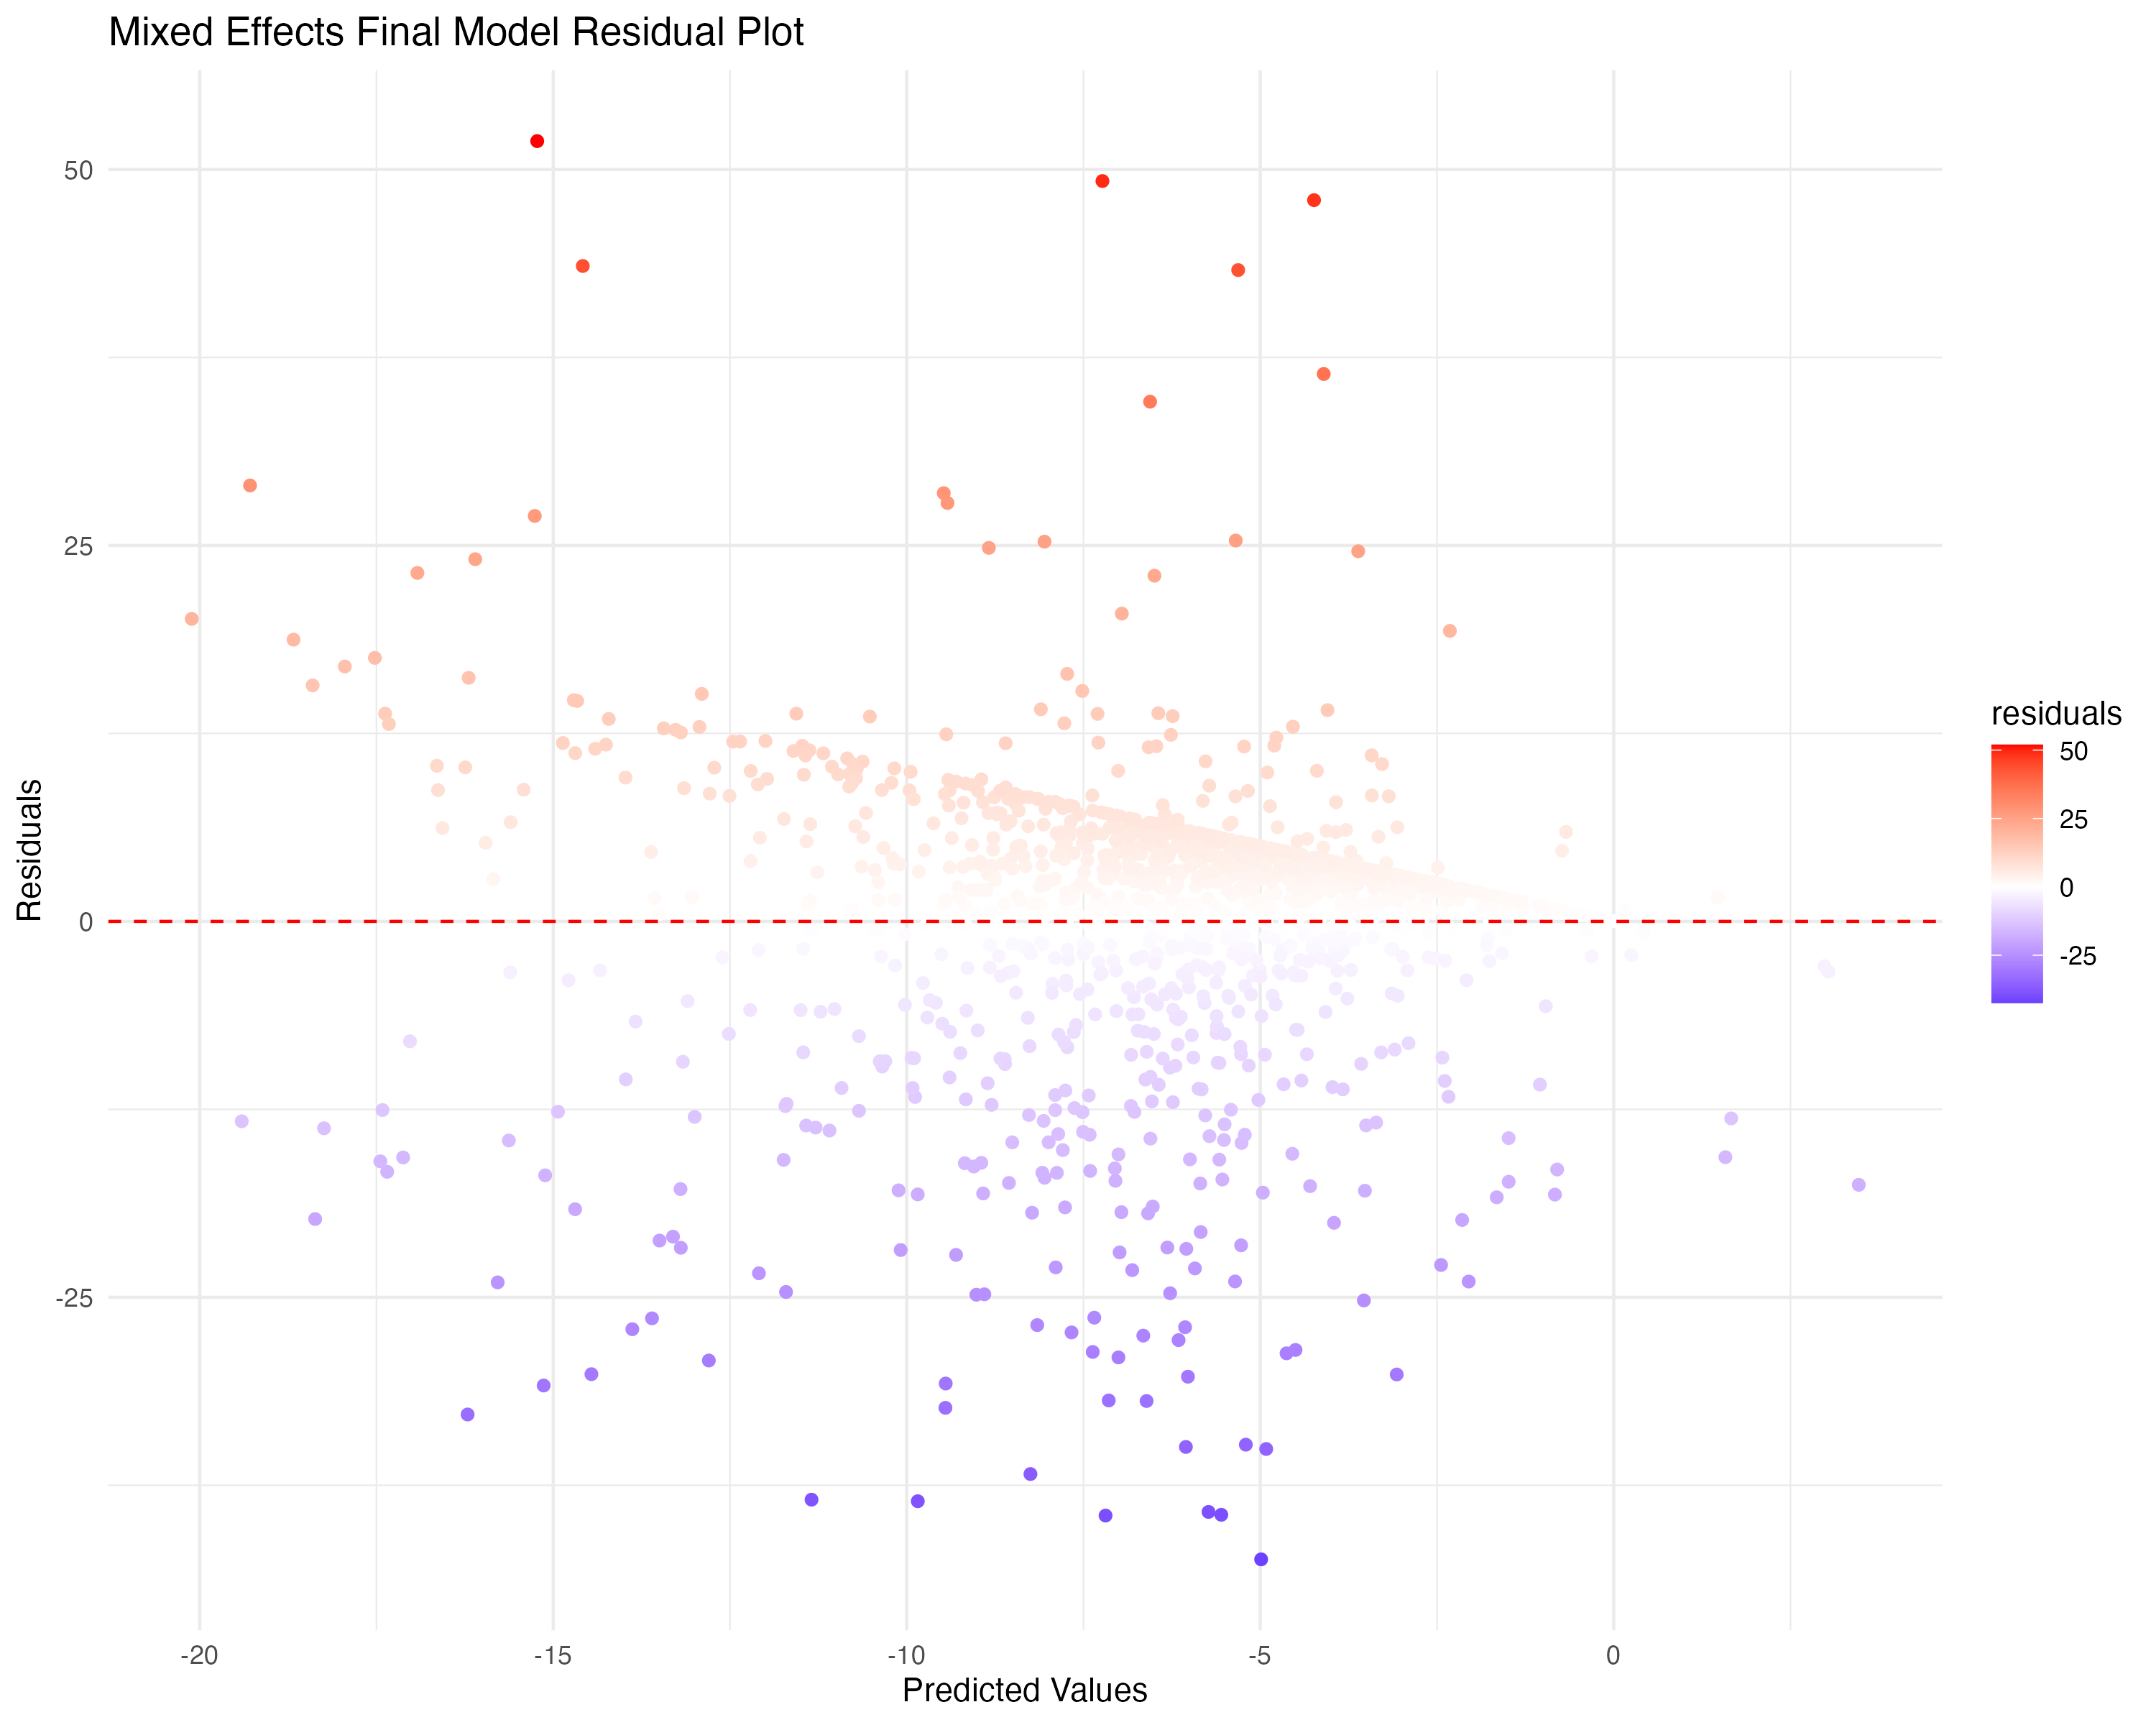
\includegraphics[width=0.8\textwidth]{figures/final_model_residuals.png}
    \caption{Mixed Effects Model Residuals Plot}
    \label{fig:mixed_effects_residuals}
\end{figure}
\noindent The residuals plot is centered around zero, which is a good sign, but there are significant outliers, especially for firms with positive change in decarbonization rate and for firms with an absolute change of more than 20\%. This suggests that the model is not performing well for these firms and it makes intuitive sense as firms who have a decarbonization rate change of more than 20\% are likely to be outliers and difficult to predict.

\section{Comparing Models Using Pycaret}
Using Pycaret \cite{pycaret}, a Machine Learning library, we will be comparing the performance of various models on the dataset. The models will be evaluated based on the RMSE, MAE, and R-squared values. The best model will be selected based on the RMSE value. We used timeseries cross-validation to ensure that the data is split in a time series fashion. As explained in the introductoiun, the folds are created using the TimeSeriesSplit method from the scikit-learn library \cite{scikit-learn}. We are not tuning the hyperparameters for the models in this section, as we will be doing that in the next section only for the best model. This analysis is useful in identifying which candidate models perform best on the dataset, and consequently which models are worth tuning.

% include table
\begin{longtable}{lrrrr}
\caption{Cross Validation Results for All Tested Models}
\label{tab:cross-validated-results}\\
\toprule
                          Model &   MAE &     MSE &  RMSE &     R2 \\
\midrule
\endfirsthead
\caption[]{Cross Validation Results for All Tested Models} \\
\toprule
                          Model &   MAE &     MSE &  RMSE &     R2 \\
\midrule
\endhead
\midrule
\multicolumn{5}{r}{{Continued on next page}} \\
\midrule
\endfoot

\bottomrule
\endlastfoot 
% color 6.91 green
                 Bayesian Ridge &  4.15 &   48.40 &  \textbf{6.91} &   0.09 \\
             CatBoost Regressor &  4.34 &   48.77 &  6.94 &   0.09 \\
               Ridge Regression &  4.22 &   48.74 &  6.94 &   0.08 \\
    Orthogonal Matching Pursuit &  4.29 &   49.09 &  6.96 &   0.08 \\
                    Elastic Net &  4.25 &   49.35 &  6.97 &   0.08 \\
               Lasso Regression &  4.23 &   49.54 &  6.99 &   0.07 \\
   Lasso Least Angle Regression &  4.23 &   49.54 &  6.99 &   0.07 \\
    Gradient Boosting Regressor &  4.34 &   49.57 &  7.00 &   0.07 \\
Light Gradient Boosting Machine &  4.35 &   49.71 &  7.01 &   0.07 \\
        Random Forest Regressor &  4.56 &   50.25 &  7.04 &   0.06 \\
          Extra Trees Regressor &  4.51 &   50.90 &  7.08 &   0.05 \\
                Dummy Regressor &  4.45 &   54.09 &  7.30 &  -0.01 \\
      Extreme Gradient Boosting &  4.85 &   57.20 &  7.51 &  -0.07 \\
          K Neighbors Regressor &  4.80 &   60.37 &  7.71 &  -0.13 \\
                Huber Regressor &  4.38 &   67.05 &  8.13 &  -0.25 \\
        Decision Tree Regressor &  5.89 &   96.97 &  9.80 &  -0.84 \\
             AdaBoost Regressor &  9.13 &  115.14 & 10.60 &  -1.12 \\
   Passive Aggressive Regressor &  6.84 &  187.64 & 12.92 &  -2.66 \\
              Linear Regression & 31.33 & 3024.39 & 35.90 & -42.10 \\
\end{longtable}


\noindent Note how Bayesian Ridge and CatBoost have the lowest RMSE values. We will be exploring these models further in the next section. In general though, no model is significantly better than the others, which suggests that there is significant unexplained variance in the data. This is to be expected, as the CDP survey data is a first step in understanding the decarbonization rate, but there are many other factors that determine the decarbonization rate, especially in the long term. Additionally, there is significant noise in the data due to inconsistent reporting, which makes it difficult to predict the decarbonization rate accurately. That is, firms may not report their decarbonization rate accurately, or they may not report it at all, which makes it difficult to predict. In this exercise, I preferred

\section{Bayesian Ridge Model}

The Bayesian Ridge model is a linear regression model that uses a Bayesian approach to estimate the coefficients of the model. The model is regularized using a prior distribution on the coefficients, which helps to prevent overfitting. The model is evaluated based on the RMSE, MAE, and R-squared values. The hyperparameters that we tuned are the alpha parameter, which controls the strength of the regularization, and the lambda parameter, which controls the strength of the prior distribution on the coefficients. The best model was selected based on the RMSE value. Train and test results are reported in the Table \ref{tab:bayesian_ridge_performance} below. 

\begin{table}[H]
    \centering
    \caption{Bayesian Ridge Model Performance Metrics for Training and Test Sets}
    \label{tab:bayesian_ridge_performance}
    \begin{tabular}{lcccc}
    \hline
    Set & $R^2$ & RMSE & MSE & MAE \\ 
    \hline
    Training & 0.9 & 6.91 & 48.4 & 4.15 \\
    Test & 0.10 & 9.59 & 91.9 & 6.46 \\
    \hline
    \end{tabular}
\end{table}
\noindent The Bayesian Ridge model has a RMSE of 9.59 on the test set, which is very similar to the Mixed Effects Model. This suggests that the Bayesian Ridge model is not significantly better than the Mixed Effects Model. 

\subsection{Feature Importance Plot}
% Feature Importance Plot
\begin{figure}[H]
    \centering
    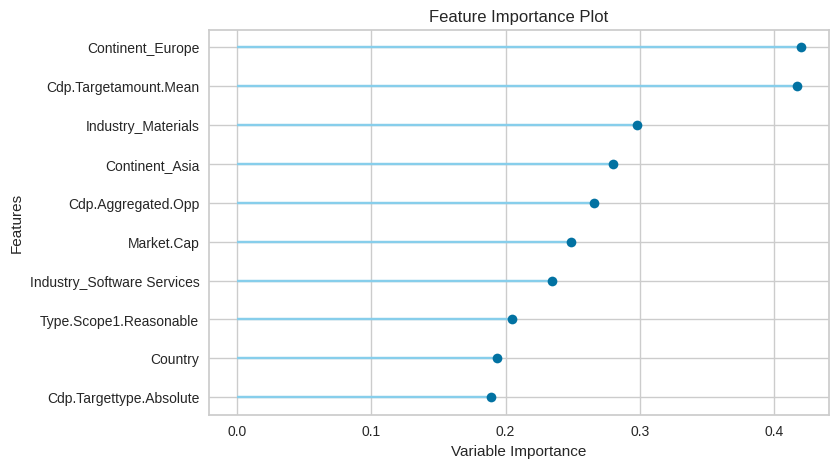
\includegraphics[width=0.8\textwidth]{figures/Bayes_Importance.png}
    \caption{Bayesian Ridge Model Feature Importance Plot}
    \label{fig:bayesian_ridge_feature_importance}
\end{figure}
The feature importance plot \ref{fig:bayesian_ridge_feature_importance} shows that the most important features are continent Europe, the Target Amount Mean, the industry Materials, whether the firm identified an opportunity to reduce emissions. All those features are consistent with the Mixed Effects Model and the Exploratory Data Analysis we performed in Chapter \ref{ch:data-sources}. Consistency across model when it comes to feature importance is a good sign, as it suggests that the features are indeed important for predicting the decarbonization rate and that they are not just artifacts of the model.

\subsection{Residuals Plot}
% Residuals Plot
\begin{figure}[H]
    \centering
    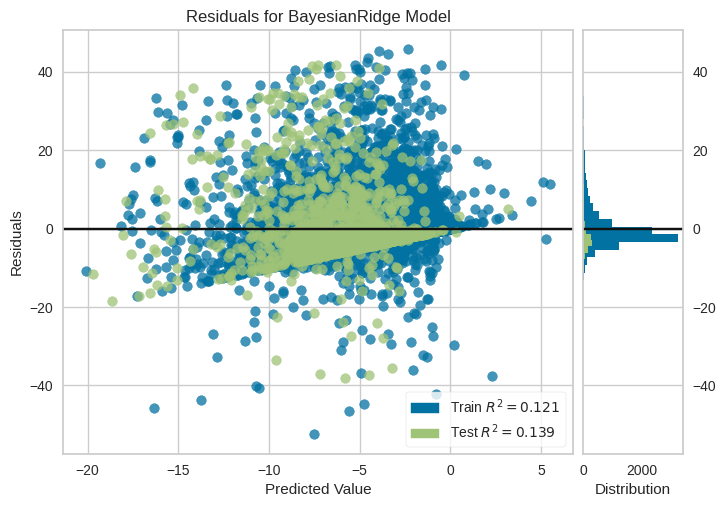
\includegraphics[width=0.8\textwidth]{figures/Bayes_Residuals.png}
    \caption{Bayesian Ridge Model Residuals Plot}
    \label{fig:bayesian_ridge_residuals}
\end{figure}

The residuals plot is smilar to the Mixed Effects Model, centered around zero, but with significant outliers, especially for firms with positive change in decarbonization rate and for firms with an absolute change of more than 20\%. This suggests that both models have similar performance and are not performing well for these firms. This makes sense and is consistent with the fact that the data is noisy and that with a greater focus on enhancing reporting quality for relevant variables, the models could be greatly improved.

\section{Catboost Regressor Model}
To tune the Catboost Regressor model, we used grid search and cross-validation to find the best hyperparameters for the model. The hyperparameters that we tuned are the learning rate, the depth of the tree, the number of trees, and the l2 regularization parameter. We used the TimeSeriesSplit method from the scikit-learn library to ensure that the data is split in a time series fashion with number of folds $cv = 3$. The model was evaluated based on the RMSE, MAE, and R-squared values. The best model was selected based on the RMSE value. The hyperparameters that we tuned are as follows:

\begin{table}[H]
    \centering
    \caption{Hyperparameters for Catboost Regressor}
    \label{tab:hyperparameters}
    \begin{tabular}{@{}lcc@{}}
    \toprule
    Parameter       & Grid of Values        & Selected Best Value \\ 
    \midrule
    Depth           & 4, 6, 8               & \textbf{6}                   \\
    Iterations      & 500, 1000             & \textbf{1000}                \\
    Learning Rate   & 0.01, 0.02, 0.03      & \textbf{0.02}                \\
    L2 Leaf Reg     & 1, 3                  & \textbf{1}                   \\ 
    \bottomrule
    \end{tabular}
\end{table}



\subsection{Model Performance Metrics}
\begin{table}[H]
    \centering
    \caption{Catboost Regressor Tuned Model Performance Metrics}
    \label{tab:catboost_regressor_performance}
    \begin{tabular}{lcccc}
    \hline
    Set & $R^2$ & RMSE & MSE & MAE \\ 
    \hline
    Training & 0.33 & 5.73 & 35.91 & 3.47 \\
    Test & 0.11 & 9.54 & 91.13 & 6.25 \\
    \hline
    \end{tabular}
\end{table}
\noindent The Catboost Regressor model has a RMSE of 9.54 on the test set, and the $R^2$ value is 0.11, which is the best performance so far. This suggests that the Catboost Regressor model is the best model for this dataset. It does not come as a surprise, as Catboost is known for its ability to handle categorical variables and its robustness to overfitting. Therefore, model performance is in line with theoretical expectations and the results from the previous chapter with the main takeaway being that the model is able to generalize well to the test set, but the noise in the response variable significantly limits predictive performance.


    

\subsection{Feature Importance Plot}

\begin{figure}[H]
    \centering
    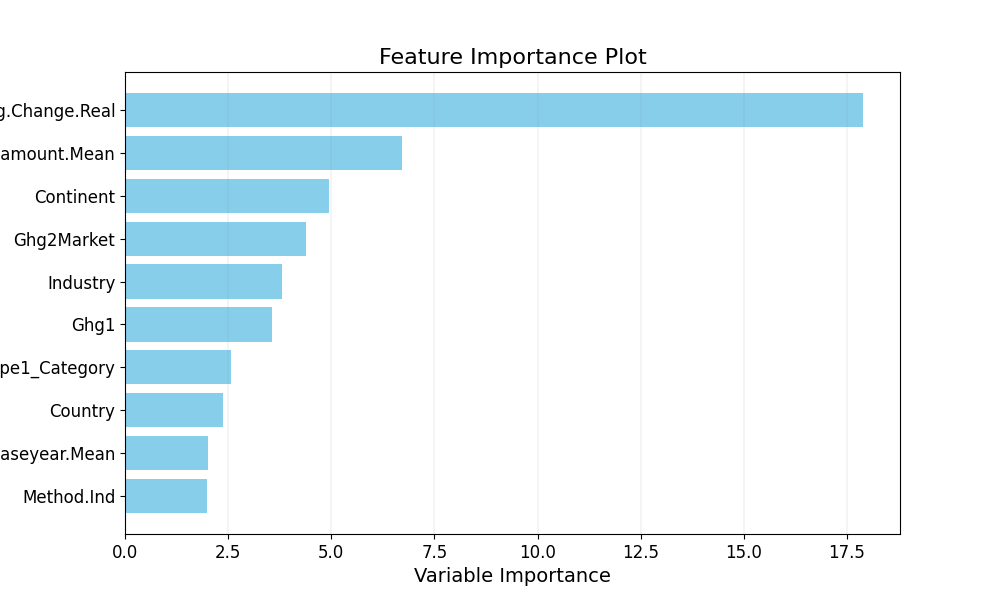
\includegraphics[width=0.8\textwidth]{figures/catboost_feature_importance.png}
    \caption{Catboost Regressor Feature Importance Plot}
    \label{fig:catboost_feature_importance}
\end{figure}
\noindent Catboost has a built-in feature importance plot, which is shown in Figure \ref{fig:catboost_feature_importance}. The most important features are the Current Decarbonization Rate Change, Target Amount Mean, Continent, Whether the firm reports market based emisisons, and the industry. Note how reassuringly all the selected features by a tree-based boosting method, which is very different from the linear models, are consistent with the Mixed Effects Model and the Bayesian Ridge Model. We therefore learn that there is a consensus across models that the most important features are the same, thus to advance our ability to predict the decarbonization rate, we should focus on these features.


\subsection{Shapley Beeswarm Values Plot}

\begin{figure}[H]
    \centering
    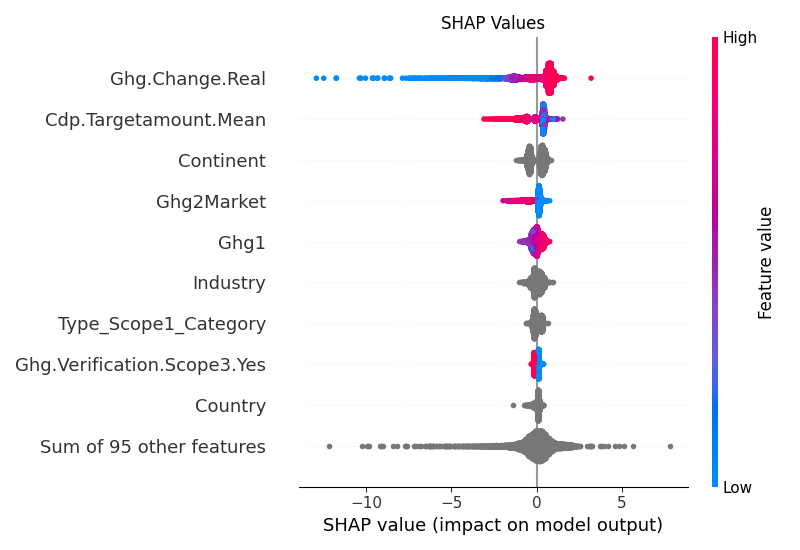
\includegraphics[width=0.8\textwidth]{figures/catboost_shap_values_beeswarm.png}
    \caption{Catboost Regressor Shapley Beeswarm Values Plot}
    \label{fig:catboost_shapley_values}
\end{figure}

For the Catboost Regressor model, we used the Shapley values to explain the predictions of the model. The Shapley values are a measure of feature importance that is based on game theory \cite{NIPS2017_7062}. The Shapley values are calculated for each feature and are used to explain the predictions of the model. The Shapley values are plotted in Figure \ref{fig:catboost_shapley_values}. The beeswarm plot shows the distribution of the Shapley values for each feature. The plot offers an interpretation of the effect that each feature has on the model's prediction, with a high Shapley value off the x-axis indicating a strong effect on the model's prediction in that direction. Therefore, the plot is useful in understanding the relationship between the features and the model's predictions akin to interpreting coefficients in a linear model. In this regard, the effect of current decarbonization rate change is important and positive, that is firms with a positive change in decarbonization rate are likely to have a higher decarbonization rate next year. Similarly, the effect of the target amount mean is important and negative, that is firms with a higher target amount mean are likely to have a better decarbonization rate next year. The effect of Scope 2 Market Emissions is also similiar to what we found in the Mixed Effects Model: firms that report market based emissions are likely to have a better decarbonization rate next year. 





